%
% CHAPTER: Interesting Research Questions
%

\chapterimage{Wikipedia_Monument_2.pdf}

\chapter{Computational Creativity}
\label{chap:computational-creativity}

\begin{quote}
\begin{flushright}
\emph{To be surprised, to wonder, \\
is to begin to understand.}\\
José Ortega y Gasset \\
\end{flushright}
\end{quote}
\bigskip

In this Chapter we are going to see how to apply in practice our methodology for the assisted discovery of interesting research questions. As it was the case of previous chapter, in which we studied the concept of nescience from a practical point of view, ...

In the first part of this chapter we will see how to approximate the new metrics introduced: relevance and applicability. The relevance of a topic will be based on the number of web pages on Internet that link to the topic's page on Wikipedia (external links), and applicability will be estimated by the number of links from the Wikipedia's scientific pages to themselves (internal links). We will provide some practical examples of both quantities for the set of topics that compose the research area of theoretical computer science. Then, we will describe how to apply in practice our methodology for the discovery of interesting questions, and we will come up with some examples of new research questions that, in principle, could be addressed by science. The new questions proposed will be both, intradisciplinary, coming from the area of theoretical computer science, and interdisciplinary, by means of combining the area of theoretical computer science with the area of philosophy and the area of biochemistry. Finally, we will derive some new interesting research topics, according to our subjective interpretation of the combinations found, that are enough interesting to deserve to be the subject of new research activities. We will also evaluate if the proposed topics fulfill the requirements that we proposed in Chapter \ref{chap:Interesting-Research-Questions} for a question to be classified as interesting.

In the last part of the chapter, we will apply the set of metrics defined for the classification of individual research topics to full research areas. In this way, we will compute the interestingness of the different research disciplines as source of new problems, and their interestingness as a source of useful tools to solve open problems. These metrics will allow us to compare the relative merits of different knowledge disciplines. Some examples of research areas in decay will be shown as well.

\section{Classification of Research Topics}

In order to evaluate the classification metrics proposed we have used the set of topics corresponding to all the categories at Level 4, from the category Level 3 \emph{theory of computation} (included in category Level 2 \emph{theoretical computer science} and category Level 1 \emph{formal sciences}).

Before to compute the new interesting questions, it is highly convenient to normalize the metrics of the topics involved in the study, otherwise, a very reduced set of topics could dominate all the questions. For the normalization process we have used the BoxCox method, that it is based on the identification of the best transformation from a family of power transformations.

{\color{red} TODO: Explain the BoxCox method} 

Also, and since these studied quantities, relevance, applicability, nescience and maturity, do not have the same scale, it is highly convenient to apply the following additional transformation:

\[
\mu_{t}^{,}=\frac{\mu_{t}-\min(\mu)}{\max(\mu)-\min(\mu)}
\]

where $\mu_t$ refers to the considered metric (nescience, relevance, ...). 

\subsection{Relevance}

In Definition \ref{def:relevance} we introduced the concept of relevance of a research topic as a measure of the impact that this topic could have in people's life. The idea was that the higher the relevance, the higher its potential as a source of interesting questions, since we would be addressing a problem that affects many people. Relevance was defined as the degree of the research topic in the relevance graph, a bipartite graph connecting topics and people (see Definition \ref{def:relevance-graph}). Of course, this relevance graph is a mathematical abstraction that it is very difficult to compute in practice, since we do not have information about how people is affected by each topic.

As an approximation of the relevance of a topic we have used the number of links (URLs) from external web pages on the whole Internet that point to the topic's web page on Wikipedia. The rationale is that the more relevant is a topic, the more people will be talking about it on Internet, and the more URLs there will be linking to Wikipedia, since Wikipedia is a well known source of information to which many people refer. In fact, we are not interested in knowing the absolute relevance of research topics, since what we need is a measure of relative relevance between different topics. An underestimate of the relevance is not harmful as long this underestimation is equally distributed among all the topics. It requires further research to fully understand how well the the theoretical concept of relevance is approximated by this URLs counting procedure. 

Another problem is that we do not know the number of links to a web page on Internet, and so, we have to apply a second approximation. In this case, the number of links was estimated using Google's \texttt{link:} facility in searches. Google's \texttt{link:} lists the links that Googlebot discovered during its crawling and indexing process of Internet. For example, the number of external pages that link to the \emph{Computer Science} article in Wikipedia is given by:

\smallskip

\texttt{
link:http://en.wikipedia.org/wiki/Computer\_science
}

\smallskip

As Google recognizes in its web page, not all links to a site may be listed. The number of links could vary due to redirections, crawling errors, and other problems. How these errors affect to the accuracy of the links counting is not clear, since the details of the Google's crawling algorithm are not public.

Figure \ref{fig:Relevance-of-Topics} shows a plot of the relevance of the set of topics after the application of the normalization process described in {\color{red} XXX}. A practical problem is that there are too many topics with a very low number of links (as indexed by Google). That should not be a problem since we are not using at any moment those topics with very low relevance.

\begin{figure}[h]
\centering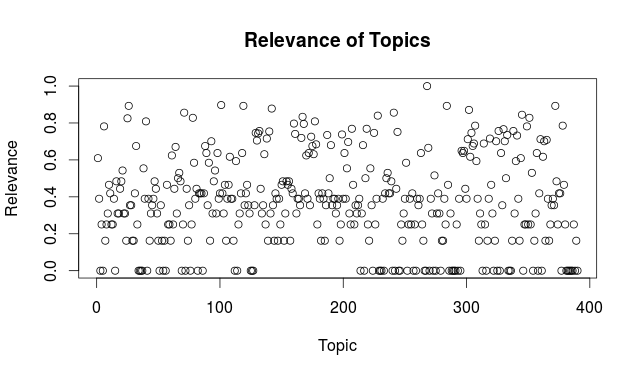
\includegraphics[scale=0.5]{RelevanceTopics}
\caption{\label{fig:Relevance-of-Topics}Relevance of topics}
\end{figure}

Table \ref{tab:Relevance-of-Topics} contains the ten most relevant topics according to its relevance. For each topic it is shown it relevance (number or external links) and the normalized version of this number. The list includes basic concepts (\emph{binary number,} \emph{floating point}), advanced concepts (\emph{Turing machine}, \emph{finite-state machine, cellular automaton, lambda calculus}, \emph{Turing completeness}), highly popular tools (\emph{recursion}, \emph{regular expression}) and classical problems (\emph{halting problem}). All those topics could fit into our intuitive idea of highly relevant, although some authors could perfectly disagree that some of them are the most relevant ones in the area of theory of computation (for example, \emph{floating point}).

\begin{table}
\begin{centering}
\begin{tabular}{|c|c|c|}
\hline 
Topic & Relevance & Norm.\tabularnewline
\hline 
\hline 
Regular expression & 409 & 1.00\tabularnewline
\hline 
Turing machine & 159 & 0.90\tabularnewline
\hline 
Binary number & 141 & 0.89\tabularnewline
\hline 
Recursion & 133 & 0.88\tabularnewline
\hline 
Finite-state machine & 118 & 0.86\tabularnewline
\hline 
Halting problem & 108 & 0.85\tabularnewline
\hline 
Cellular automaton & 104 & 0.85\tabularnewline
\hline 
Floating point & 99 & 0.84\tabularnewline
\hline 
Lambda calculus & 95 & 0.84\tabularnewline
\hline 
Turing completeness & 93 & 0.83\tabularnewline
\hline 
\end{tabular}
\par\end{centering}

\caption{\label{tab:Relevance-of-Topics}Relevance of topics}
\end{table}

\subsection{Applicability}

Applicability measures how likely is that a research topic can be applied to solve open problems. If a tool has been already applied to solve multiple problems, then there is a high probability that it can be used again to solve new problems. The number of problems in which a tool has been applied is computed with the aid of the applicability graph (see Definiton \ref{def:applicability-graph}), and applicability is formally defined as the out-degree of the topic in this graph (see Definiton \ref{def:applicability}). We have approximated the applicability graph by means of using the graph of internal links between the scientific pages of Wikpiedia. That is, we approximate the applicability of a topic by counting the number of pages from Wikipedia domain that links to the topic's page (we have used the \emph{``What links here''} facility from Wikipedia, a tool to see the list of the pages that link to, or redirect to, the current page). As it was the case of the relevance of a topic, we are not intersted in the absolute value of the applicability of topics. What it is important for us is the relative ordering of topics based on their applicability. Perhaps, a better approach to approximate the applicability of a topic would be to analyze the graph of citations from academic research papers, combined with the automatic identification of the topics addressed in those papers.

% TODO: Perhaps we could include a nice picture of the graph of Wikipedia internal links

The applicability of a topic Figure \ref{fig:Applicability-of-Topics} shows a plot of the applicability of the selected set of topics after the normalization process, and Table \ref{tab:Applicability-of-Topics} contains the ten most relevant topics according to its applicability. For each topic it is shown the number or internal links and the normalized version of this number. In the list we can find topics like \emph{regular expression}, \emph{recursion}, \emph{Turing machine}, or \emph{cellular automaton} that perfectly fits our intuitive idea of tools that can be applied to solve other problems. However, we can also find in the list the topic \emph{quantum computer} that is not very applicable, but since it is a highly popular research topic it is mentioned in many different Wikipedia's pages. Other pages like \emph{division by zero}, \emph{floating point}, or \emph{binary number}, do not seems to be good tools either. The final topic, \emph{computatibility theory}, shows that, even at the fourth level, we still can find too broad topics.

\begin{figure}[h]
\centering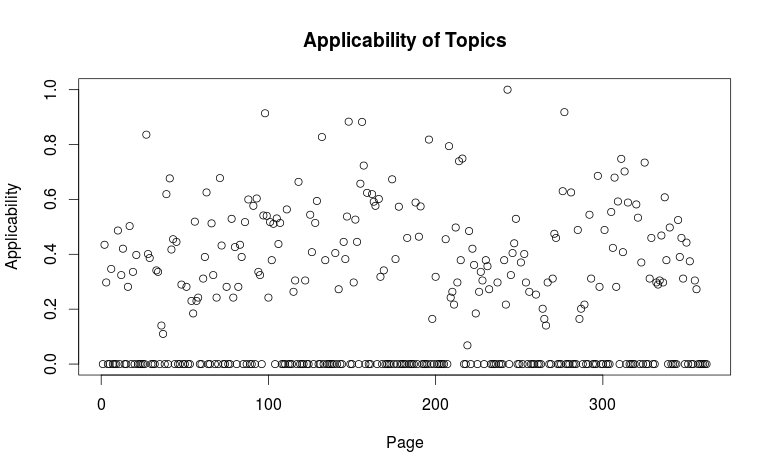
\includegraphics[scale=0.5]{ApplicabilityTopics}
\caption{\label{fig:Applicability-of-Topics}Applicability of topics}
\end{figure}

\begin{table}
\begin{centering}
\begin{tabular}{|c|c|c|}
\hline 
Topic & Applicab. & Norm.\tabularnewline
\hline 
\hline 
Regular expression & 1971 & 1.00\tabularnewline
\hline 
Recursion & 1227 & 0.91\tabularnewline
\hline 
Quantum computer & 1197 & 0.91\tabularnewline
\hline 
Division by zero & 998 & 0.88\tabularnewline
\hline 
Floating point & 992 & 0.88\tabularnewline
\hline 
Turing machine & 748 & 0.83\tabularnewline
\hline 
Binary number & 710 & 0.82\tabularnewline
\hline 
Ternary num. sys. & 670 & 0.80\tabularnewline
\hline 
Cellular automaton & 433 & 0.74\tabularnewline
\hline 
Computability theory & 430 & 0.73\tabularnewline
\hline 
\end{tabular}
\par\end{centering}

\caption{\label{tab:Applicability-of-Topics}Applicability of topics}
\end{table}

\subsection{Maturity}

\section{Interesting Research Questions}

\subsection{Intradisciplinary Questions}

\subsection{Interdisciplinary Questions}

\section{New Research Topics}

\section{Classification of Research Areas}

\section{References}

Papers about the BoxCox method ...

\section{Future Work}


